\begin{center}\large\textbf{Readings: 13.1-13.6 584-633}\\
\normalsize \end{center}
\large \hlinewd{2pt}
~\\
We've looked at one-way ANOVA so far.  This models the $t$ treatments using $t-1$ degrees of freedom.  However, the treatments may actually be combinations of more than 1 factor of interest.  What we'll be able to do now is answer the question, which factor(s) (not treatment(s)) are important!\\~\\

\textbf{A multiway ANOVA example}\\
An observational study was done to investigate the Cholesterol levels of different groups of people.  There were two factors in this experiment
\begin{itemize}
\item Age - levels = Younger than 50 (Young), Older than 50 (Old)
\item Gender - levels = Male, Female
\end{itemize}
Therefore, we have 2x2=4 treatments.  Label the treatments as
\begin{itemize}
\item OF = Old Female (group 1)
\item OM = Old Male (group 2)
\item YF = Young Female (group 3)
\item YM = Young Male (group 4)
\end{itemize}
Within each treatment group we have $n_j=n=7$ observations (a balanced design).  To investigate if any treatment means differ, we can do a One-Way ANOVA analysis by fitting the model
$$Y_{ij} = \mu + \tau_i + E_{ij}$$
where $i=1 (OF),2 (OM),3 (YF),4 (YM)$, $j=1,2,\ldots,7$ and $E_{ij}$ i.i.d. $N(0,\sigma^2)$.  We constrain that $\sum_{i=1}^{t}\tau_i=0$. \\~\\
The data and One-Way ANOVA output are given below:
\begin{center}
\begin{tabular}{c|ccccccc|cc} \hline
Treatment & \multicolumn{7}{c}{Cholesterol level}& avg & std. dev. \\ \hline
OF (i=1) & 262 & 193 & 224 & 201 & 161 & 178 & 265 & $\bar{y}_{1+}=212.0$& $s_{1}=40$\\ 
OM (i=2) & 192 & 253 & 248 & 278 & 232 & 267 & 289 & $\bar{y}_{2+}=251.3$& $s_{2}=32$\\ 
YF (i=3) & 221 & 213 & 202 & 183 & 185 & 197 & 162 & $\bar{y}_{3+}=194.7$ & $s_{3}=20$\\ 
YM (i=4) & 271 & 192 & 189 & 209 & 227 & 236 & 142 & $\bar{y}_{4+}=209.4$& $s_{4}=41$\\ 
 \hline
\end{tabular}
\end{center}

\begin{small}
\begin{verbatim}
proc glm data=cholesterol;
class Treatment;
model Chol=Treatment;
lsmeans Treatment/cl pdiff adjust=tukey;
run;
\end{verbatim}
\end{small}

\begin{center}
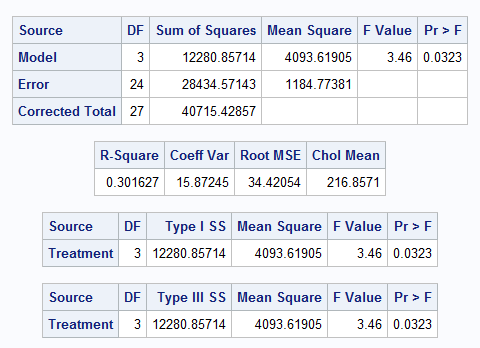
\includegraphics[scale=0.65]{CholOneWay}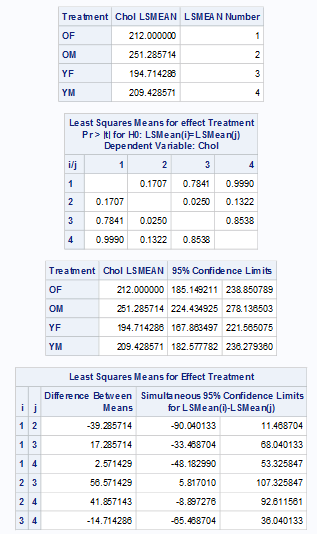
\includegraphics[scale=0.8]{CholOneWay2}
\end{center}

Conclusion from ANOVA table p-value is that the treatment means, $\mu+\tau_i$ or equivalently $\mu_i$, are not plausibly equal (using $\alpha=0.05$).  From the lsmeans statement we can see that Young Females and Old Males are the only groups that differ significantly.\\~\\

\newpage

Now suppose we want to decide what effects the Age factor and the Gender factor have on the response.  That is, rather than just inspect treatment mean differences, can we say that Age is significant for predicting Blood Pressure? What about Gender? \\~\\

We can investigate these by looking at contrasts!  Consider the plots below:
\begin{center}
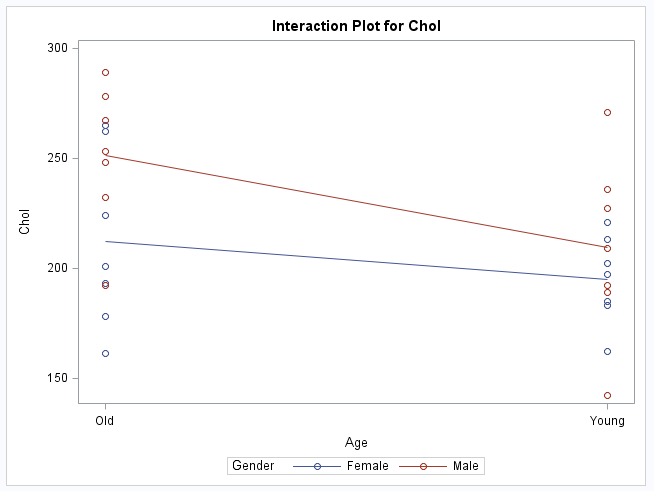
\includegraphics[scale=0.5]{CholIntPlot1}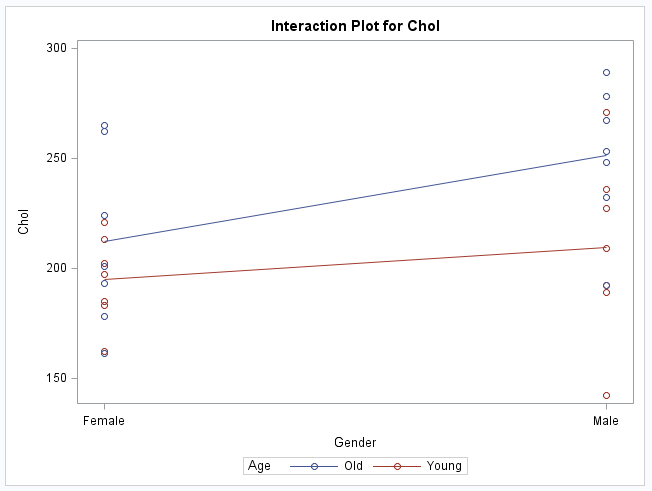
\includegraphics[scale=0.5]{CholIntPlot2}
\end{center}

The \textbf{main effect} of factor A is the change in the response for switching levels of factor A (averaged over all other factors).\\
What contrast would test for the \textit{main effect} of Age?\\~\\
$\theta_{Age} = $\\~\\~\\
What contrast would test for the \textit{main effect} of Gender?\\~\\
$\theta_{Gender} = $\\~\\~\\
There is a third contrast of interest.  This contrast represents the \textbf{interaction} between Age and Gender.\\~\\
An \textbf{interaction} between factor A and factor B implies that the effect of factor A on the response depends on the level of factor B (and vice-versa).\\~\\
In terms of the plots above, Age and Gender interact if the lines are not parallel (can look at either plot).  What contrast can we write to investigate this?\\~\\
$\theta_{Age*Gender} = $

\newpage

\begin{enumerate}
\item Check that $\theta_{Age}$, $\theta_{Gender}$, and $\theta_{Age*Gender}$ are mutually orthogonal.  \\~\\~\\~\\
\item Use the previous output to find estimates for each contrast and provide standard errors.  Recall: $\hat\theta=\sum c_i \bar{y}_{i+}$ and $\hat{SE}(\hat{\theta})=\sqrt{MS(E)\sum_{i=1}^{t}\frac{c_i^2}{n_i}}$\\~\\~\\
$\hat{\theta}_{Age} = $\\~\\~\\
$\hat{\theta}_{Gender} = $\\~\\~\\
$\hat{\theta}_{Age*Gender} = $\\
\item Find the sums of squares for each contrast.  How many degrees of freedom are associated with each contrast?   Recall: $ SS(\hat\theta) = \frac{\hat\theta^2}{\sum \frac{c_i^2}{n_i}}.$\\~\\~\\
$SS(\hat{\theta}_{Age}) = $\\~\\~\\
$SS(\hat{\theta}_{Gender}) = $\\~\\~\\
$SS(\hat{\theta}_{Age*Gender}) = $\\
\item Formulate a test of $H_0:\theta_i=0$ for each of these three contrasts.  Obtain the $F$-ratio for each of these tests. Compare them to the F-critical value $F(1,24,0.05)=4.26)$ and make a decision about the importance of each effect.\\~\\~\\
$F_{Age}=\underbar{~~~~~~~~~~~~~~~~~~~~~~~~~~~~~~~~}~~~~~num~df=\underbar{~~~~~~~}~~den~df=\underbar{~~~~~~~}$\\~\\~\\
$F_{Gender}=\underbar{~~~~~~~~~~~~~~~~~~~~~~~~~~~~~~~~}~~~~~num~df=\underbar{~~~~~~~}~~den~df=\underbar{~~~~~~~}$\\~\\~\\
$F_{Age*Gender}=\underbar{~~~~~~~~~~~~~~~~~~~~~~~~~~~~~~~~}~~~~~num~df=\underbar{~~~~~~~}~~den~df=\underbar{~~~~~~~}$
\item What do you notice about the sum of these sums of squares?  Find the F-statistic for a test of $H_0:\theta_{Age}=\theta_{Gender}=\theta_{Age*Gender}=0$ vs $H_A:$ at least one differs.  What do you notice about this test and the overall F-test from the ANOVA table in the One-Way model?\\~\\~\\~\\~\\~\\~\\~\\
\end{enumerate}
Notice what we've done:  Very similar to partitioning the $SS(Tot)$ into $SS(Model)$ and $SS(E)$, we've partitioned $SS(Trt)$, which has $t-1=4-1=3$ degrees of freedom into 3 independent components that represent different effects of interest!  We can test for each effect to learn more about our factors rather than just the treatment means.\\~\\~\\
This is the idea of Multi-Way ANOVA!  (Although it gets a little bit more complicated when a factor has more than 2 levels.)\\~\\~\\
Let's look at how we could get these contrasts in SAS:
\begin{small}
\begin{verbatim}
proc glm data=cholesterol;  class Treatment;  model Chol=Treatment;
contrast 'Age Main Effect Contrast' intercept 0 treatment 0.5 0.5 -0.5 -0.5;
contrast 'Gender Main Effect Contrast' intercept 0 treatment 0.5 -0.5 0.5 -0.5;
contrast 'Age*Gender Interaction Effect Contrast' intercept 0 treatment 0.5 -0.5 -0.5 0.5;
estimate 'Age Main Effect Estimate' intercept 0 treatment 0.5 0.5 -0.5 -0.5;
estimate 'Gender Main Effect Estimate' intercept 0 treatment 0.5 -0.5 0.5 -0.5;
estimate 'Age*Gender Interaction Effect Estimate' intercept 0 treatment 0.5 -0.5 -0.5 0.5;  run;
\end{verbatim}
\end{small}

\begin{center}
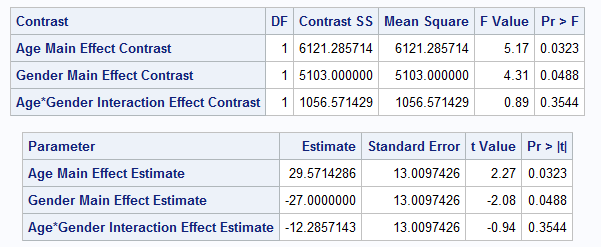
\includegraphics[scale=0.75]{CholContrasts}
\end{center}

\newpage

Using the estimate and contrast statements in One-Way ANOVA:\\
We need to write our contrast in terms of the model parameters $\mu$, $\tau_1, \tau_2,\tau_3$, and $\tau_4$. \\~\\
For instance, 
$$\theta_{Gender}=\frac{1}{2}(\mu_1+\mu_3)-\frac{1}{2}(\mu_2+\mu_4)=\frac{1}{2}(\mu+\tau_1+\mu+\tau_3-\mu-\tau_2-\mu-\tau_4)$$
$$=0\mu+\frac{1}{2}\tau_1-\frac{1}{2}\tau_2+\frac{1}{2}\tau_3-\frac{1}{2}\tau_4$$
In terms of syntax, we write contrast or estimate followed by a name to distinguish it.  Then we do
\begin{center}
intercept \underbar{coef on $\mu$}~~~treatment \underbar{coef on $\tau_1$}~~\underbar{coef on $\tau_2$}~~\underbar{coef on $\tau_3$}~~\underbar{coef on $\tau_4$}
\end{center}
A contrast statements will give you the contrast sum of squares and a p-value.\\~\\
An estimate statement will estimate any `estimable' function of parameters (coefficients don't have to sum to 0). 

\newpage
\textbf{Two-Way ANOVA example}\\~\\
Rather than fit a One-Way ANOVA model, we can use a different parameterization of that model called a Two-Way ANOVA model.\\~\\
The Two-Way ANOVA model for the cholesterol measurements is:
$$Y_{ijk} = \mu + \alpha_i + \beta_j + (\alpha \beta)_{ij} + E_{ijk}$$
$i=1,2 (old,young)$~~~$j=1,2 (female, male)$ and $k=1,2,\ldots,7$.\\
We still assume $E_{ijk} \iid N(0,\sigma^2)$.  With parameter constraints:
$$\alpha_1+\alpha_2=0, \beta_1+\beta_2=0,\mbox{ and }$$
$$(\alpha\beta)_{11}+(\alpha\beta)_{12}=0,(\alpha\beta)_{21}+(\alpha\beta)_{22}=0,(\alpha\beta)_{11}+(\alpha\beta)_{21}=0,(\alpha\beta)_{12}+(\alpha\beta)_{22}=0$$~\\
This is called a 2$\times$2 design since we have 2 factors with 2 levels each and the treatments are found by \textit{crossing} the levels of the factors.  (A three factor design with 2, 3, and 5 levels would be a 2$\times$3$\times$5 design.)
\begin{itemize}
\item $Y_{ijk}$ is the response for replicate $k$ at level $i$ of Age and level $j$ of Gender
\item $\mu$ represents the overall mean of cholesterol, 
$$\mbox{estimate is }\hat{\mu}=\bar{Y}_{+++}$$
\item $\alpha_i$ represents the `effect' for being at level $i$ of Age, 
$$\mbox{estimate is }\hat{\alpha}_i=\bar{Y}_{i++}-\bar{Y}_{+++}$$
\item $\beta_i$ represents the `effect' for being at level $j$ of Gender, 
$$\mbox{estimate is }\hat{\beta}_j=\bar{Y}_{+j+}-\bar{Y}_{+++}$$
\item $(\alpha\beta)_{ij}$ represents the `joint effect' for being at level $i$ of Age and level $j$ of Gender, 
$$\mbox{estimate is }\hat{(\alpha\beta)}_{ij}=\bar{Y}_{ij+}-\bar{Y}_{i++}-\bar{Y}_{+j+}+\bar{Y}_{+++}$$
\item $E_{ijk}$ is a random error\\~\\
\end{itemize}
For level $i$ of Age and level $j$ of Gender we are model the mean cholesterol as
$$\mu_{ij}=\mu(A_{i}B_{j})=E(Y_{ijk})=\mu+\alpha_i+\beta_j+(\alpha\beta)_{ij}$$
and, as you might expect, the estimate for level $i$ of Age and level $j$ of Gender is
$$\hat{\mu_{ij}}=\widehat{\mu(A_{i}B_{j})}=\bar{Y}_{+++}+(\bar{Y}_{i++}-\bar{Y}_{+++})+(\bar{Y}_{+j+}-\bar{Y}_{+++})+(\bar{Y}_{ij+}-\bar{Y}_{i++}-\bar{Y}_{+j+}+\bar{Y}_{+++}) =\bar{Y}_{ij+}$$

\newpage

The two-way ANOVA model can be fit easily in proc glm using the following code:
\begin{small}
\begin{verbatim}
proc glm data=cholesterol;
class Age Gender;
model Chol=Age Gender Age*Gender; 
run;
\end{verbatim}
\end{small}

\begin{center}
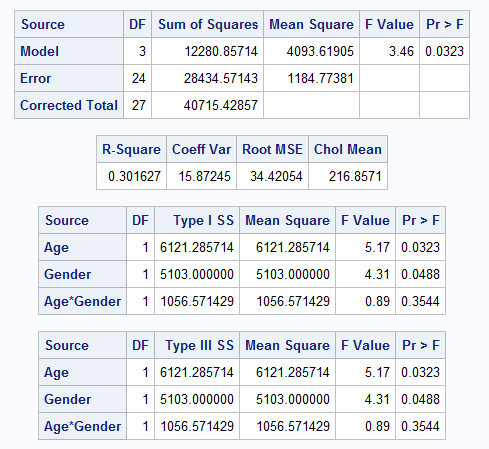
\includegraphics[scale=0.75]{CholTwoWay}
\end{center}

The sums of squares for each effect are equal to the sums of squares for our contrasts in the one-way ANOVA model.\\~\\~\\
When looking at Two-Way ANOVA output,
\begin{enumerate}
\item Inspect the overall ANOVA table p-value.  If significant,
\item Inspect the interaction p-value.  
\begin{enumerate}
\item If significant, both factors are important for predicting the response (why?).
\item If not significant, investigate the main effect p-values for significance to determine which factors are important for predicting the response.
\end{enumerate}
\end{enumerate}

\newpage


\textbf{Types of Effects Investigated}
There are three basic effects that are usually of interest in Two-way ANOVA:
\begin{itemize}
\item Simple Effects
\item Main Effects
\item Interaction Effects
\end{itemize}
Use this table of means from the cholesterol example in the following questions:
\begin{center}
\begin{tabular}{c|cc}
&~~~~Gender\\
&female(j=1) &male(j=2)\\\hline
Age Older (i=1) & $\hat{\mu}_{11}$=212.0 (previously $\hat{\mu}_{1}$)& $\hat{\mu}_{12}$=251.3 (previously $\hat{\mu}_{2}$)\\
~~~~~Young (i=2) & $\hat{\mu}_{21}$=194.7 (previously $\hat{\mu}_{3}$)& $\hat{\mu}_{22}$=209.4 (previously $\hat{\mu}_{4}$)
\end{tabular}
\end{center}

\begin{enumerate}
\item If we denote the mean for a level combination as $\mu_{ij}$ or $\mu(A_iB_j)$ (i.e. mean at factor A level $i$ and factor B level $b$), how many different means are we attempting to estimate in a 2$\times$2 Two-way ANOVA design?  How many means in a general a$\times$b Two-way ANOVA design?\\~\\~\\~\\
\item \textbf{Simple Effects}\\
\begin{enumerate}
\item In the 2$\times$2 set-up, a simple effect for factor A is the difference in the level means of factor A \textit{at a given level of factor B}.  That is,
$$\text{Simple effect of A at level }1\text{ of B is defined as }\mu[AB_1]=\mu(A_2B_1)-\mu(A_1B_1)=\mu_{21}-\mu_{11},$$ 
$$\text{Simple effect of A at level }2\text{ of B is defined as }\mu[AB_2]=\mu(A_2B_2)-\mu(A_1B_2)=\mu_{22}-\mu_{12},$$ 
\item Define the simple effects of factor B.\\~\\~\\~\\~\\~\\
\item For the Cholesterol example, estimate these four simple effects and explain what each measures.
\end{enumerate}
\newpage

\item \textbf{Main Effects}
\begin{enumerate}
\item Main effects in a 2x2 experiment are the averages of the simple effects.  Define the main effect of factor A as
$$\mu[A]=\frac{1}{2}(\mu[AB_1]+\mu[AB_2])=\frac{1}{2}(\mu_{22}-\mu_{12}+\mu_{21}-\mu_{11})=\frac{1}{2}(\mu_{22}+\mu_{21})-\frac{1}{2}(\mu_{12}+\mu_{11})$$
Our $\theta_{Age}$ contrast from before!
\item Define the main effect for factor B.\\~\\~\\~\\~\\
*****Main effects should (usually) only be looked at when interaction effects are not significant.\\
\item For the Cholesterol example, estimate these two main effects and explain what each measures.\\~\\~\\~\\~\\
\end{enumerate}

\item \textbf{Interaction Effects}
\begin{enumerate}
\item Interaction effects in a 2x2 experiment are the average of the \textit{difference} of simple effects.  If nonzero, this implies that when the level of factor B is changed, factor A acts differently with respect to the response.  Define the interaction between factor A and B as
$$\mu[AB]=\frac{1}{2}(\mu[AB_2]-\mu[AB_1])=\frac{1}{2}(\mu_{22}-\mu_{12}-\mu_{21}+\mu_{11}).$$
Our $\theta_{Age*Gender}$ contrast from before!
\item Show the average of the difference of simple effects for factor B yields the same answer as above.\\~\\~\\~\\
\item For the Cholesterol example, estimate this interaction effect and explain what it measures.
\newpage
\item Interactions are easily seen in a 2x2 experiment by looking at an 'interaction plot'.  
\begin{enumerate}
\item If an interaction effect causes the relationship between the levels of a factor to change, this is called a \textbf{qualitative} interaction.  
\item If the interaction effect just changes the magnitude of the relationship between the levels of a factor, this is called a \textbf{quantitative} interaction.
\end{enumerate}
\item Label the plots below accordingly:
\begin{center}
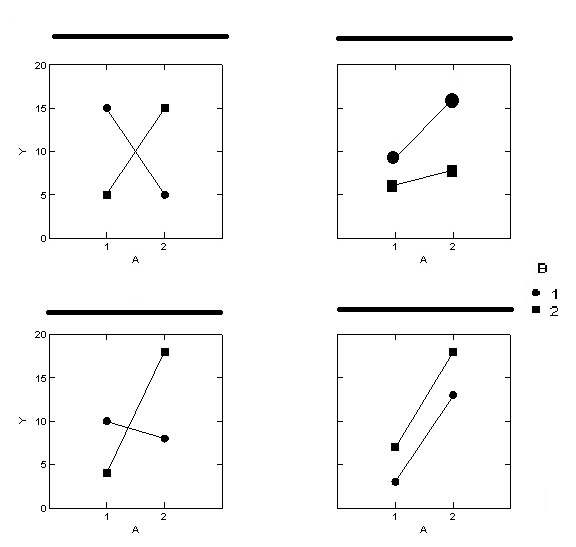
\includegraphics[height=3.4in,width=5in]{interact}
\end{center}
\item If interactions exist, looking at main effects is usually not necessary.  For example, approximately what would the main effect for factor A be equal to for the top left plot?\textbf{An interaction implies both factors are important!}  \\~\\~\\~\\~\\
\end{enumerate}
\end{enumerate}

\newpage

To test for the Age main effect notice, 
\begin{eqnarray*}
\hat{\mu}[A]&=&\frac{1}{2}(\hat{\mu}_{22}-\hat{\mu}_{12}+\hat{\mu}_{21}-\hat{\mu}_{11})\\
&= & \frac{1}{2}(\bar{Y}_{22+}-\bar{Y}_{12+}+\bar{Y}_{21+}-\bar{Y}_{11+})\\
& = & \frac{1}{2}(\bar{Y}_{22+}+\bar{Y}_{21+})-\frac{1}{2}(\bar{Y}_{12+}+\bar{Y}_{11+})\\
& = & \bar{Y}_{2++}-\bar{Y}_{1++} \\
&=& \hat{\alpha}_{2}-\hat{\alpha}_{1}
\end{eqnarray*}
Our test for the main effect of Age can be written as
$$H_0: \alpha_{1}=\alpha_{2}=0\mbox{ vs } H_A:\mbox{ At least 1 is not 0}$$~\\~\\
Similarly, we can test for the Gender main effect by
$$H_0: \beta_{1}=\beta_{2}=0\mbox{ vs } H_A:\mbox{ At least 1 is not 0}$$~\\~\\
And we can test the interaction using 
$$H_0: (\alpha\beta)_{11}=(\alpha\beta)_{12}=(\alpha\beta)_{21}=(\alpha\beta)_{22}=0\mbox{ vs } H_A:\mbox{ At least 1 is not 0}$$~\\~\\
Thus, this parameterization of the model gives a very nice way to test for these different effects.

\newpage
\textbf{The general Two-Way ANOVA model:}\\
Suppose we have a \textit{continuous} response, $Y$, and two factors, A and B.  Factor A has $a$ levels and factor B has $b$ levels.  Our main interest lies in whether or not the response differs due to the factors. \\~\\
Most experiments with multiple factors we will look at will have a \textbf{factorial} treatment structure.  This implies `treatments' are combinations of the levels of different factors (also called a crossed design).  For the most part we will have \textbf{complete} experiments (i.e. observations at each level combination).  \\~\\
This particular experiment would be an a$\times$b experiment.  The parametrization of the Two-way ANOVA model we will use is
$$Y_{ijk}=\mu+\alpha_{i}+\beta_{j}+(\alpha\beta)_{ij}+E_{ijk},~~i=1,...,a,~~j=1,...,b,k=1,...,n \mbox{ balanced design}$$
with normality assumption on the errors and sum to zero constraints on the parameters (to get a unique solution).\\~\\~\\
To construct the ANOVA table, we will still take the total sum of squares and split it up.  Now we split it into a few more parts than previous:
\begin{center}
ANOVA table for a$\times$b experiment with $N=abn$ = total \# of obs\\~\\
\begin{tabular}{c|llll}
Source & df & Sum of Squares (SS) & MS\\\hline
A & $a-1$ & $SS(A)= \sum_i \sum_j \sum_k (\tmean{i+}-\gmeann)^2$ & SS(A)/(a-1)\\
B & $b-1$ & $SS(B)= \sum_i \sum_j \sum_k (\tmean{+j}-\gmeann)^2$ & SS(B)/(b-1) \\
AB & $(a-1)(b-1)$ & $SS(AB)= \sum_i \sum_j \sum_k (\tmean{ij}-\tmean{i+}-\tmean{+j}+\gmeann)^2$ & SS(AB)/((a-1)(b-1)) \\
Error & $ab(n-1)$ & $SS(E)=\sum_i \sum_j \sum_k (y_{ijk}-\tmean{ij})^2$ & SS(E)/(ab(n-1))\\
Total & $N-1$ & $SS(Tot)= \sum_i \sum_j \sum_k (y_{ijk}-\gmeann)^2$ & \\
\end{tabular}
\end{center}

The F-statistics are given by $MS(A)/MS(E)$, $MS(B)/MS(E)$, and $MS(AB)/MS(E)$ respectively.  \\~\\
Note: $SS(A)+SS(B)+SS(AB) = SS(Trt)$ in One-Way ANOVA\\~\\
$(a-1)+(b-1)+(a-1)(b-1)=t-1$ (degrees of freedom in One-Way ANOVA)\\~\\
We still have that $SS(A)+SS(B)+SS(AB)+SS(E)=SS(Tot)$ and same for the degrees of freedom.

\newpage

\textbf{An a$\times$b example}\\
An entomologist records energy expended ($y$) by $N=27$ honeybees at $a=3$ temperature ($A$) levels ($20,30,40^o C$) consuming liquids with $b=2$ levels of sucrose concentration ($B$)$(20\%,40\%)$ in a balanced, completely randomized crossed $3 \times 2$ design.  The data are given below:
\begin{center}
\begin{tabular}{|cc|ccc|}  \hline
Temp & Suc & \multicolumn{3}{c|}{Sample} \\ \hline
   20 & 20 & 3.1 & 3.7 & 4.7 \\
   20 & 40 & 5.5 & 6.7 & 7.3 \\
   30 & 20 & 6 & 6.9 & 7.5 \\
   30 & 40 & 11.5 & 12.9 & 13.4 \\
   40 & 20 & 7.7 & 8.3 & 9.5 \\
   40 & 40 & 15.7 & 14.3 & 15.9 \\\hline
\end{tabular}
\end{center}

\begin{small}
\begin{verbatim}
proc glm data=ent;
class Temp Suc;
model Energy=Temp|Suc; *Vertical Bar fits all combinations of Temp and Suc (main effects and interactions);
run;
\end{verbatim}
\end{small}

\begin{center}
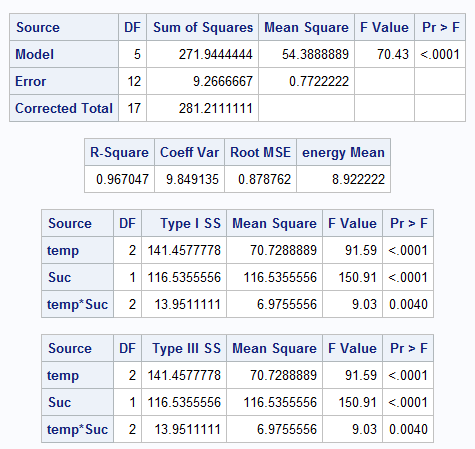
\includegraphics[scale=0.6]{Ent}
\end{center}

Unlike a $2\times2$ study, it is not possible to express interaction between Temp and Suc using 1 contrast.\\~\\
Likewise, we can't estimate the main effect of Temp with only 1 contrast!\\~\\

\newpage

\begin{small}
\begin{verbatim}
title 'Means for each treatment group';
proc tabulate data=ent;
class Temp Suc;
var Energy;
table Temp*mean, Energy*Suc;
run;
\end{verbatim}
\end{small}

\begin{center}
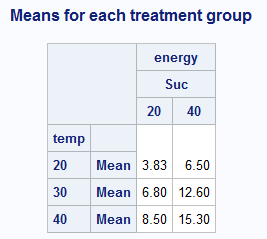
\includegraphics[scale=0.9]{EntMeans}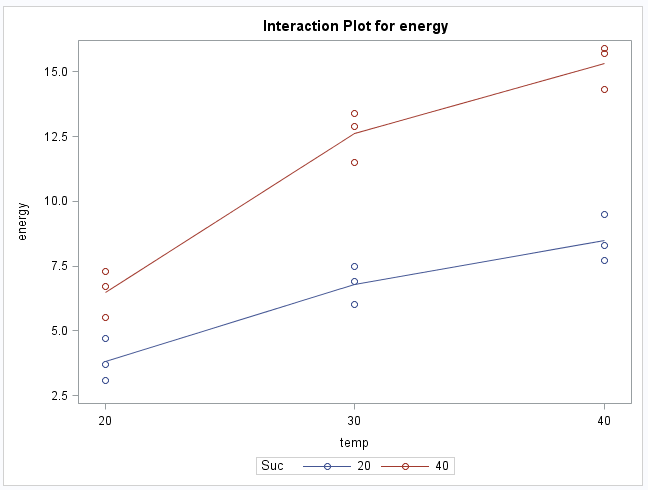
\includegraphics[scale=0.6]{Ent2}
\end{center}

\textbf{Testing Interaction in an $a \times b$ experiment}\\
Here we have (3-1)(2-1)=2 degrees of freedom for interaction.  Why?  Well, no interaction implies changing the level of Temp doesn't change the effect of Suc on Energy, i.e.
$$\mu_{12}-\mu_{11}=\mu_{22}-\mu_{21}\mbox{ or }\mu_{Temp20,Suc40}-\mu_{Temp20,Suc20}=\mu_{Temp30,Suc40}-\mu_{Temp30,Suc20}$$
as well as
$$\mu_{12}-\mu_{11}=\mu_{32}-\mu_{31}\mbox{ or }\mu_{Temp20,Suc40}-\mu_{Temp20,Suc20}=\mu_{Temp40,Suc40}-\mu_{Temp40,Suc20}$$
as well as
$$\mu_{32}-\mu_{31}=\mu_{22}-\mu_{21}\mbox{ or }\mu_{Temp40,Suc40}-\mu_{Temp40,Suc20}=\mu_{Temp30,Suc40}-\mu_{Temp30,Suc20}$$
But notice that given any two of these contrasts (move all means to one side to see these as a contrast), we can get the third contrast.  So we have 3-1=2 contrasts that are needed for testing interaction.\\~\\
Again, no interaction would imply \textbf{piecewise parallel lines} across all the levels of the factor on the axis.\\~\\

Test for interaction effect generalizes as:
$$ H_0: (\alpha \beta)_{ij} \equiv 0 \mbox{ vs. }  H_1: (\alpha \beta)_{ij} \neq 0 \mbox{ for some } i,j$$
$$ F=\frac{MS(AB)}{MS(E)}$$
on $(a-1)(b-1)$ numerator and $abn-ab$ denominator $df$.  \\~\\

For honeybee data, 
$$ SS(AB) = n \sum_{i=1}^3 \sum_{j=1}^2 (\bar{y}_{ij+} - \bar{y}_{i++} - \bar{y}_{+j+} + \bar{y}_{+++} )^2 = 13.95 $$
which is highly significant ($p=0.004$) on 2 and 12 degrees of freedom.\\~\\
Note:  These three contrasts are not orthogonal to one another so we could not use them to find $SS(AB)$, we would have to find 2 orthogonal contrasts that represent this effect.\\~\\

%Relating this to contrasts, we can define
%$$\theta_{int1}=\mu_{21}-\mu_{11}-\mu_{22}+\mu_{12}$$
%$$\theta_{int2}=\mu_{31}-\mu_{11}-\mu_{32}+\mu_{12}$$
%$$\theta_{int3}=\mu_{31}-\mu_{21}-\mu_{32}+\mu_{22}$$
%hen 
%$$SS(\hat{\theta}_{int1})=\frac{(6.8-3.83-12.6+6.50)^2}{1^2/3+(-1)^2/3+(-1)^2/3+1^2/3}=7.348$$
%$$SS(\hat{\theta}_{int2})=\frac{(8.5-3.83-15.3+6.50)^2}{1^2/3+(-1)^2/3+(-1)^2/3+1^2/3}=12.793$$
%$$SS(\hat{\theta}_{int3})=\frac{(8.5-6.8-15.3+12.6)^2}{1^2/3+(-1)^2/3+(-1)^2/3+1^2/3}=0.75$$
%and now we can find $SS(AB)$ by doing multiplying by the appropriate factor
%$$SS(AB)=(SS(\hat{\theta}_{int1})+SS(\hat{\theta}_{int2})+SS(\hat{\theta}_{int3}))(2/3)=13.93$$~\\~\\
Since we have a significant interaction, our next step would be to analyze \textbf{simple effects} of each factor.  That is, we would investigate the effects of Temperature at given levels of Sucrose and also looking at the effect of Sucrose at given levels of Temperature.  This can be done in SAS:

\begin{small}
\begin{verbatim}
proc glm data=ent; class Temp Suc;
model Energy=Temp|Suc;
lsmeans Temp*Suc/adjust=tukey pdiff cl; run;
\end{verbatim}
\end{small}

\begin{center}
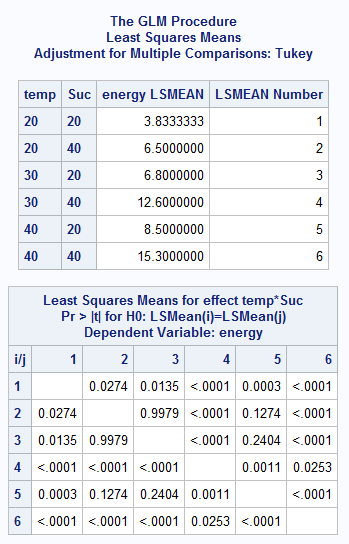
\includegraphics[scale=0.7]{EntDiffs}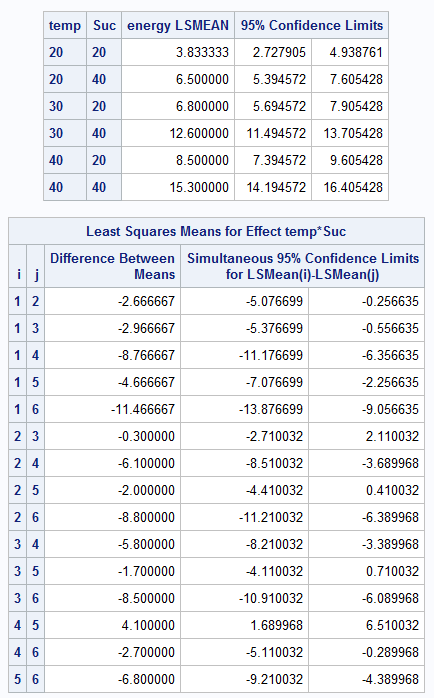
\includegraphics[scale=0.7]{EntDiffs2}
\end{center}

In reality, we would probably only be interested in simple effects such as Temp 20, Suc 40 vs Temp 20, Suc 20 (i.e. the effect of Suc, holding temperature at 20).  We could write estimate or contrast to get just those, but this is easier.\\~\\~\\

We could proceed to test for main effects, but we won't.  Why not?\\~\\~\\~\\
If one insists on main effects, the appropriate $F$-ratios are
$$ F_A = \frac{SS(A)/(a-1)}{MS(E)} \mbox { on }a-1,N-ab \ \ df $$
$$ F_B = \frac{SS(B)/(b-1)}{MS(E)} \mbox { on }b-1,N-ab \ \ df$$ ~\\

Testing of the Sucrose main effect would be done just as before since we have only two levels, we would look at the marginal means of sucrose and compare them.\\~\\
Testing of the Temperature main effect requires a bit more, we want to compare the three levels of temperature (20, 30, 40):
$$\frac{1}{2}(\mu_{21}+\mu_{22})=\frac{1}{2}(\mu_{11}+\mu_{12}) \mbox{ or }\frac{1}{2}(\mu_{Temp30,Suc20}+\mu_{Temp30,Suc40})=\frac{1}{2}(\mu_{Temp20,Suc20}+\mu_{Temp20,Suc40})$$
as well as
$$\frac{1}{2}(\mu_{31}+\mu_{32})=\frac{1}{2}(\mu_{11}+\mu_{12}) \mbox{ or }\frac{1}{2}(\mu_{Temp40,Suc20}+\mu_{Temp40,Suc40})=\frac{1}{2}(\mu_{Temp20,Suc20}+\mu_{Temp20,Suc40})$$
as well as
$$\frac{1}{2}(\mu_{31}+\mu_{32})=\frac{1}{2}(\mu_{21}+\mu_{22}) \mbox{ or }\frac{1}{2}(\mu_{Temp40,Suc20}+\mu_{Temp40,Suc40})=\frac{1}{2}(\mu_{Temp30,Suc20}+\mu_{Temp30,Suc40})$$
Again, given any two of these we can find the third so we really only need 2 contrasts ($df = 3-1 = 2$).

\newpage
\textbf{Another $a \times b$ Design - Interaction Not Significant}
\bigkn 
Yields on $36$ tomato crops from balanced, complete, crossed design with $a=3$ varieties ($A$) at $b=4$ planting densities ($B$) :
\begin{center}
\begin{tabular}{|cc|ccc|}  \hline
Variety & Density $k/hectare$ & \multicolumn{3}{c|}{Sample} \\ \hline
1 & 10 & 7.9 & 9.2 & 10.5 \\
2 & 10 & 8.1 & 8.6 & 10.1 \\
3 & 10 & 15.3 & 16.1 & 17.5 \\
1 & 20 & 11.2 & 12.8 & 13.3 \\
2 & 20 & 11.5 & 12.7 & 13.7 \\
3 & 20 & 16.6 & 18.5 & 19.2 \\
1 & 30 & 12.1 & 12.6 & 14.0 \\
2 & 30 & 13.7 & 14.4 & 15.4 \\
3 & 30 & 18.0 & 20.8 & 21.0 \\
1 & 40 & 9.1 & 10.8 & 12.5 \\
2 & 40 & 11.3 & 12.5 & 14.5 \\
3 & 40 & 17.2 & 18.4 & 18.9 \\ \hline
\end{tabular}
\end{center}

\begin{small}
\begin{verbatim}
proc glm data=tomato; class variety density;
model Yield=Variety|Density;
lsmeans Variety Density/adjust=tukey cl; *adjust=tukey tells sas to do pdiff; run;
\end{verbatim}
\end{small}

\begin{center}
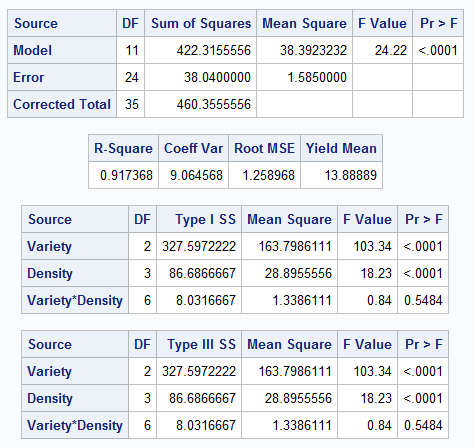
\includegraphics[scale=0.65]{Tomato1}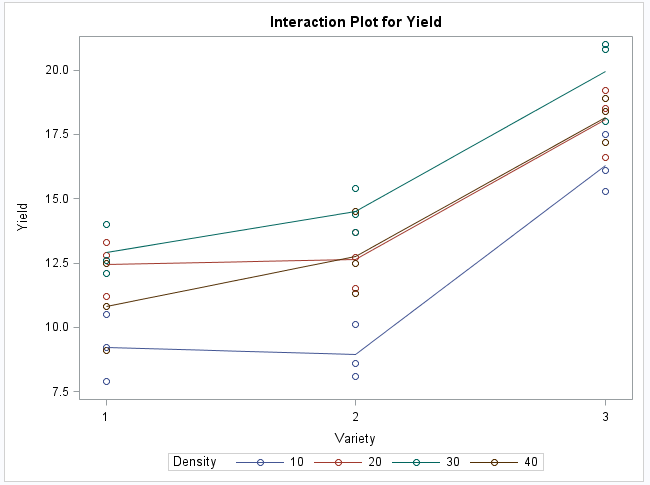
\includegraphics[scale=0.5]{Tomato2}\\
\end{center}

As the interaction is not significant we want to look at main effects p-values.  These are significant for both factors, thus both are important.  We should now look at the main effect differences for both factors (since both are important, we would not look at differences for a factor deemed non-significant).
\begin{center}
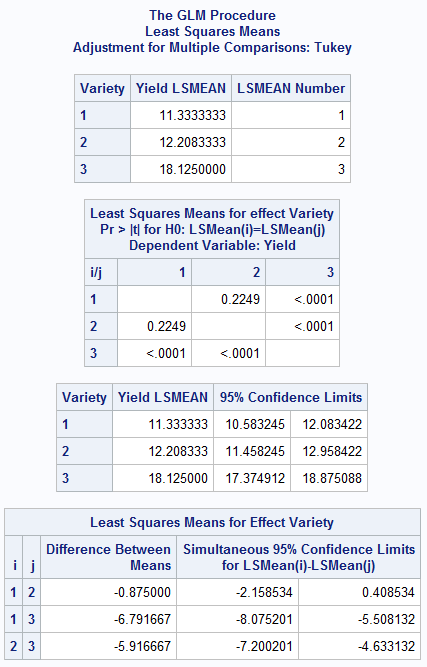
\includegraphics[scale=0.7]{Tomato3}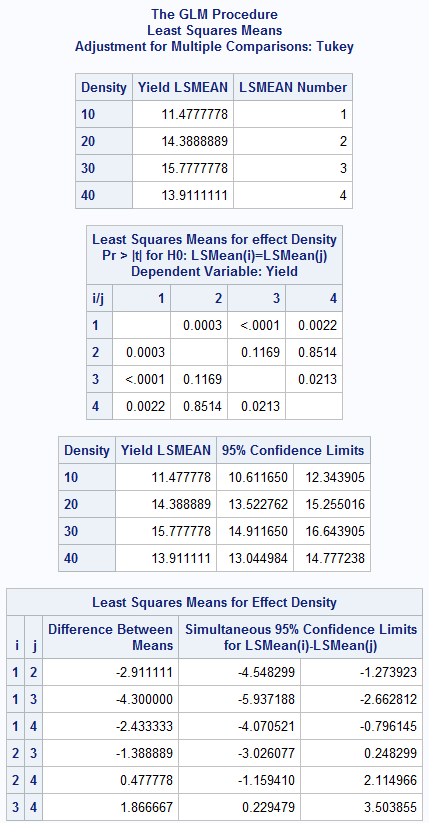
\includegraphics[scale=0.7]{Tomato4}
\end{center}

Again, analysis of replicated two (or more) factor designs often proceed according to the following directions:
\begin{enumerate}
\item Check for interaction
\item If no interaction, analyze main effects
\item If interaction, analyze simple effects
\end{enumerate}

\newpage
\textbf{A three-factor example:}
In a balanced, complete, crossed design, $N=36$ shrimp were randomized to $abc=12$ treatment combinations from the factors below:
\begin{tabbing}
A1: \= Density of shrimp population at  10\% \kill
A1: \> Temperature at $25^o$ C \\
A2: \> Temperature at $35^o$ C \\
B1: \> Density of shrimp population at 80 shrimp/$40l$ \\
B2: \> Density of shrimp population at 160 shrimp/$40l$ \\
C1: \> Salinity at 10 units \\
C2: \> Salinity at 25 units \\
C3: \> Salinity at 40 units 
\end{tabbing}
Thus, this is a 2$\times$2$\times$3 experiment.  The response variable of interest is weight gain $Y_{ijkl}$ after
four weeks.
$$Y_{ijkl} = \mu + \alpha_i + \beta_j + \gamma_k + (\alpha \beta)_{ij} + (\alpha \gamma)_{ik} + (\beta \gamma)_{jk}  + (\alpha \beta \gamma)_{ijk} + E_{ijkl}$$
where 
$$i = 1,2, ~~~j=1,2,~~~k=1,2,3,~~~l=1,2,3$$
$E_{ijkl} \iid N(0,\sigma^2).$  Note:  Many constraints are required on the parameters.\\~\\

Analysis of a Multi-Way ANOVA model starts by investigating the highest order interactions and working down from there.\\~\\

\begin{small}
\begin{verbatim}
proc glm data=shrimp; class Temp Density Salinity;
model y=Temp|Density|Salinity; run;
\end{verbatim}
\end{small}

\begin{center}
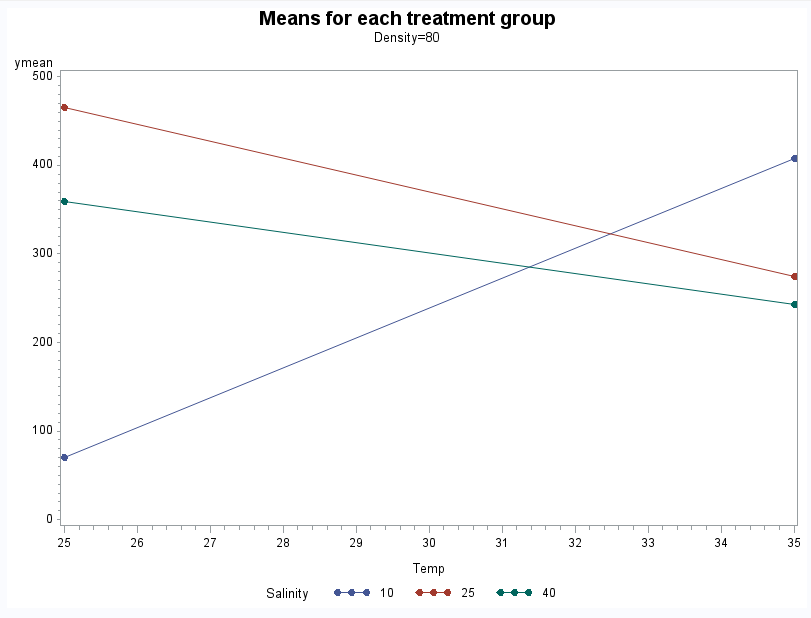
\includegraphics[scale=0.35]{Shrimp1}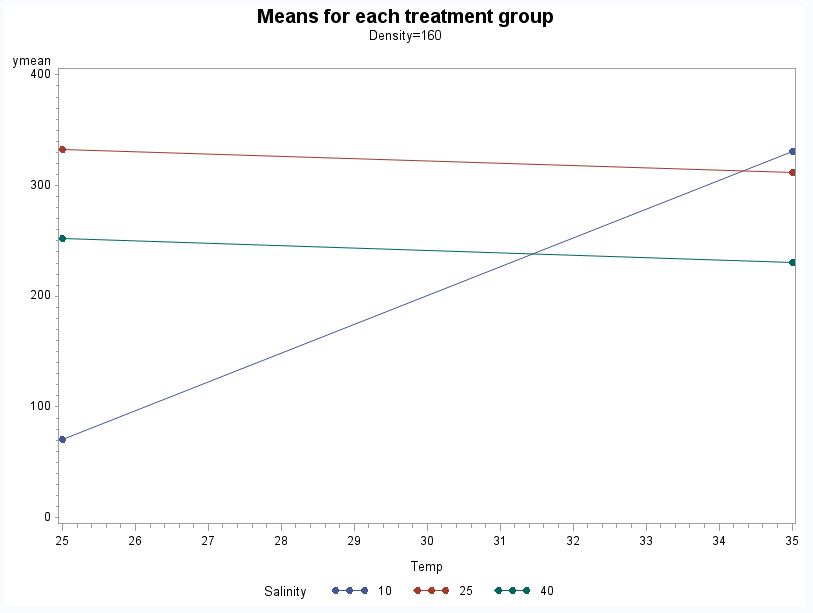
\includegraphics[scale=0.35]{Shrimp2}\\
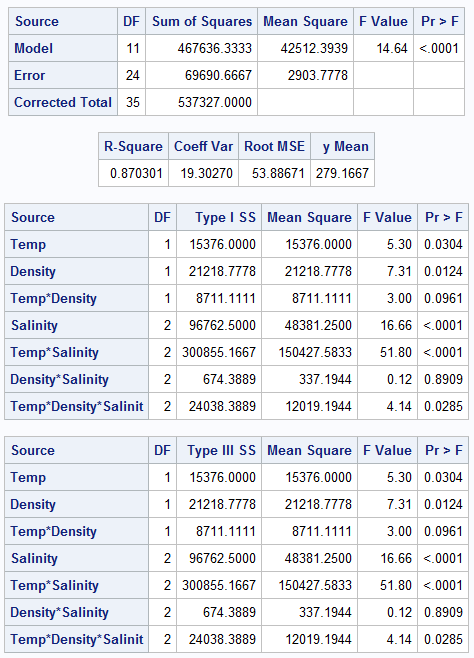
\includegraphics[scale=0.7]{Shrimp}
\end{center}

Three-way interaction is significant implying that all three factors are important.  We would now look at simple effects.  For example, the effect of temperature at density 80 and salinity 10.

\newpage

\textbf{Interpretation of second order interaction}\\~\\
\textbf{$1^{st}$ order} interaction (or two-way interaction) is between two factors \\
\textbf{$2^{nd}$ order} interaction (or three-way interaction) is between three factors, etc.\\~\\ 

Consider the $AB$ interaction at each of three levels, $C1,C2,C3$. \\~\\
To do this, look at three $2 \times 2$ tables as follows: 
\begin{center}
\begin{tabular}{cc|cc|}
&& \multicolumn{2}{c}{B} \\
\multicolumn{2}{c|}{$(C=1)$} & B1 & B2 \\ \hline
A & A1 & 70 & 71 \\
  & A2 & 408 & 331 \\ \hline
\end{tabular} \\

\begin{tabular}{cc|cc|}
&& \multicolumn{2}{c}{B} \\
\multicolumn{2}{c|}{$(C=2)$} & B1 & B2 \\ \hline
A & A1 & 466 & 333 \\
  & A2 & 275 & 312 \\ \hline
\end{tabular} \\

\begin{tabular}{cc|cc|}
&& \multicolumn{2}{c}{B} \\
\multicolumn{2}{c|}{$(C=3)$} & B1 & B2 \\ \hline
A & A1 & 359.0 & 252 \\
  & A2 & 243 & 231 \\ \hline
\end{tabular}
\end{center}

Q: How is the ABC interaction manifested here?\\~\\
A: We could compute $\hat\mu(ABC_1),\hat\mu(ABC_2),\hat\mu(ABC_3)$ and see if these first order interactions, with $C$ fixed, are the same.  (We know they are not by the $F_{ABC}$ ratio and $p$-value.)

$$\hat\mu(ABC_1) = 408-70-(331-71) \approx 77$$

Exercise: Obtain $\hat\mu(ABC_2)$ and $\hat\mu(ABC_3)$ as well as AB interaction plots for $C=1$, $C=2$ and $C=3$. 

